\documentclass{beamer}
\usepackage[english]{babel}
\usepackage{amsmath,amssymb,graphicx}

%%%%%%%%%% Start TeXmacs macros
\newcommand{\cdummy}{\cdot}
\newcommand{\mathd}{\mathrm{d}}
\newcommand{\nospace}{}
\newcommand{\tmmathbf}[1]{\ensuremath{\boldsymbol{#1}}}
\newcommand{\tmop}[1]{\ensuremath{\operatorname{#1}}}
%%%%%%%%%% End TeXmacs macros

\begin{document}

{\screens{\begin{frame}
  \
  
  \
  
  \
  
  \
  
  \
  
  \title{计算视觉与模式识别}
  
  \maketitle
  
  \ 
\end{frame}}{\begin{frame}
  \frametitle{对极几何}
  
  \resizebox{1\columnwidth}{!}{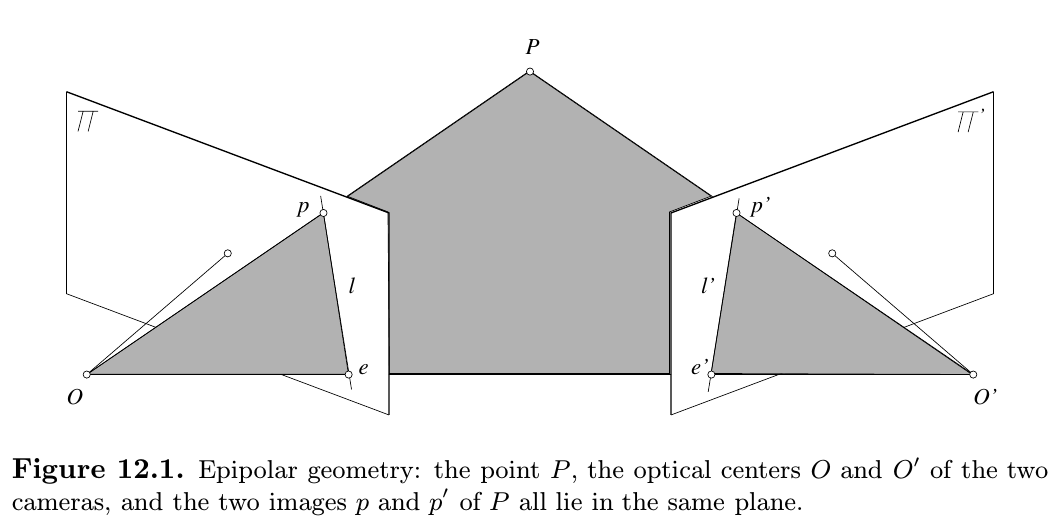
\includegraphics{img/epipolar_geometry.png}}
\end{frame}}{\begin{frame}
  \frametitle{对极约束}
  
  \resizebox{1\columnwidth}{!}{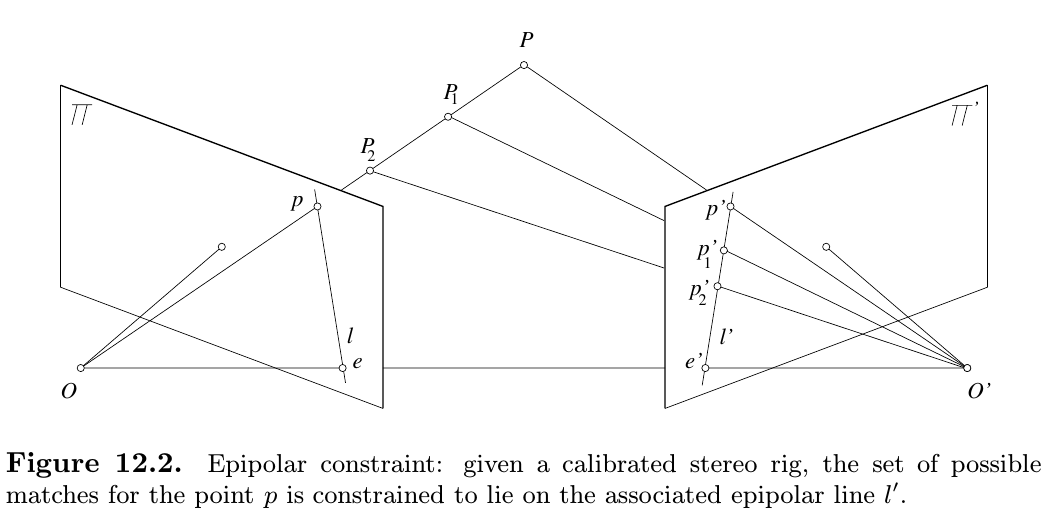
\includegraphics{img/epipolar_constraint.png}}
\end{frame}}{\begin{frame}
  \frametitle{本质矩阵}
  \begin{eqnarray*}
    \overrightarrow{\tmop{Op}} \cdummy [\overrightarrow{\tmop{OO}'} \times
    \overrightarrow{O' p'}] & = & 0\\
    \tmmathbf{p} \cdummy [\tmmathbf{t} \times (\mathcal{R}\tmmathbf{p}')] & =
    & 0\\
    \mathcal{M} & = & \left(\begin{array}{cc}
      I & \tmmathbf{0}
    \end{array}\right)\\
    \mathcal{M}' & = & \left(\begin{array}{cc}
      \mathcal{R}^T & -\mathcal{R}\tmmathbf{t}
    \end{array}\right)\\
    \tmmathbf{p} & = & \left(\begin{array}{ccc}
      u & v & 1
    \end{array}\right)^T\\
    \tmmathbf{p}' & = & \left(\begin{array}{ccc}
      u' & v' & 1
    \end{array}\right)^T
  \end{eqnarray*}
  得
  \begin{eqnarray*}
    \tmmathbf{p}^T \mathcal{E}\tmmathbf{p}' & = & 0
  \end{eqnarray*}
  其中
  \begin{eqnarray*}
    \mathcal{E} & = & [\tmmathbf{t}]_{\times} \mathcal{R}
  \end{eqnarray*}
\end{frame}}{\begin{frame}
  \frametitle{微小运动}
  \begin{eqnarray*}
    f (s) & = & \tmmathbf{p}^T [\tmmathbf{t} (s)]_{\times} \mathcal{R} (s)
    \tmmathbf{p}' (s)\\
    & = & 0
  \end{eqnarray*}
  where
  \begin{eqnarray*}
    \tmmathbf{t} (s) & = & s\tmmathbf{v}\\
    \mathcal{R} (s) & = & \tmmathbf{I}+ s [\tmmathbf{\omega}]_{\times}\\
    \tmmathbf{p}' (s) & = & \tmmathbf{p}+ s \dot{\tmmathbf{p}}
  \end{eqnarray*}
\end{frame}}{\begin{frame}
  
  \begin{eqnarray*}
    \frac{\mathd}{\mathd s} f (s) & = & \tmmathbf{p}^T [\tmmathbf{v}]_{\times}
    (\tmmathbf{I}+ s [\tmmathbf{\omega}]_{\times}) (\tmmathbf{p}+ s
    \dot{\tmmathbf{p}}) +\tmmathbf{p}^T [s\tmmathbf{v}]_{\times}
    [\tmmathbf{\omega}]_{\times} (\tmmathbf{p}+ s \dot{\tmmathbf{p}})\\
    &  & +\tmmathbf{p}^T [s\tmmathbf{v}]_{\times} (\tmmathbf{I}+ s
    [\tmmathbf{\omega}]_{\times}) \dot{\tmmathbf{p}}\\
    \left. \frac{\mathd}{\mathd s} f (s) \right|_{s = 0} & = & \tmmathbf{p}^T
    [\tmmathbf{v}]_{\times} \tmmathbf{p}\\
    & = & 0\\
    \left. \frac{\mathd^2}{\mathd s^2} f (s) \right|_{s = 0} & = &
    \tmmathbf{p}^T [\tmmathbf{v}]_{\times} [\tmmathbf{\omega}]_{\times}
    \tmmathbf{p}+\tmmathbf{p}^T [\tmmathbf{v}]_{\times} \dot{\tmmathbf{p}}
    +\tmmathbf{p}^T [\tmmathbf{v}]_{\times} [\tmmathbf{\omega}]_{\times}
    \tmmathbf{p}+\tmmathbf{p}^T [\tmmathbf{v}]_{\times} \dot{\tmmathbf{p}}\\
    & = & 2 (\tmmathbf{p}^T [\tmmathbf{v}]_{\times}
    [\tmmathbf{\omega}]_{\times} \tmmathbf{p}+\tmmathbf{p}^T
    [\tmmathbf{v}]_{\times} \dot{\tmmathbf{p}})
  \end{eqnarray*}
  得
  \begin{eqnarray*}
    \tmmathbf{p}^T [\tmmathbf{v}]_{\times} [\tmmathbf{\omega}]_{\times}
    \tmmathbf{p}+\tmmathbf{p}^T [\tmmathbf{v}]_{\times} \dot{\tmmathbf{p}} & =
    & 0
  \end{eqnarray*}
\end{frame}}{\begin{frame}
  \frametitle{平动}
  
  \resizebox{1\columnwidth}{!}{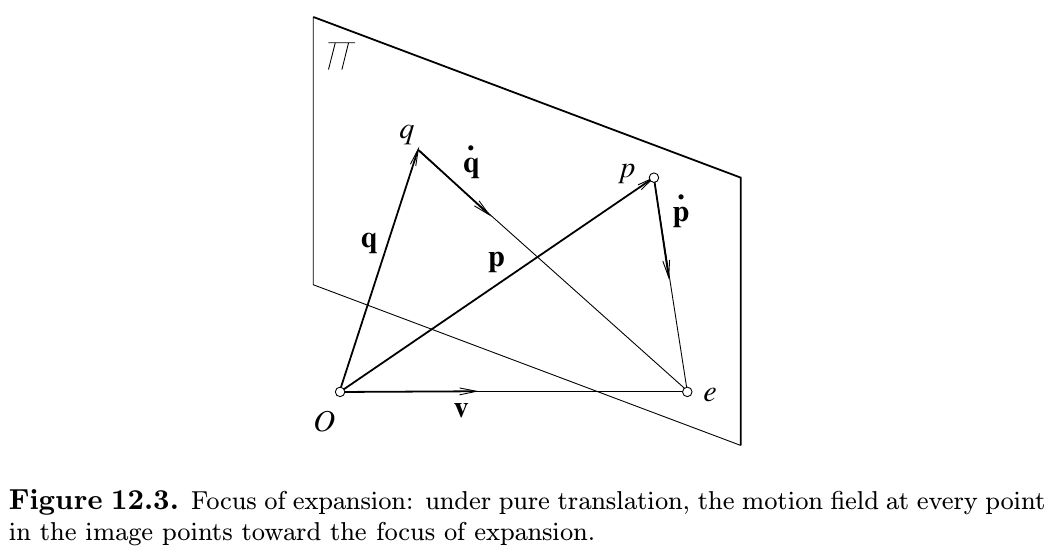
\includegraphics{img/focus_of_expansion.png}}
\end{frame}}{\begin{frame}
  \frametitle{基础矩阵}
  
  
  \begin{eqnarray*}
    \tmmathbf{p}\mathcal{F}\tmmathbf{p}' & = & 0
  \end{eqnarray*}
  where
  \begin{eqnarray*}
    \tmmathbf{p} & = & \mathcal{K} \hat{\tmmathbf{p}}\\
    \tmmathbf{p}' & = & \mathcal{K}' \hat{\tmmathbf{p}}'\\
    \mathcal{F} & = & \mathcal{K}^{- T} {\mathcal{E}\mathcal{K}'}^{- 1}
  \end{eqnarray*}
  \begin{eqnarray*}
    \mathcal{F} & = & \left(\begin{array}{ccc}
      b & a & - a \beta - b \alpha\\
      - d & - c & c \beta + d \alpha\\
      d \beta' - b \alpha' & c \beta' - a \alpha' & - c \beta \beta' - d
      \beta' \alpha + a \beta \alpha' + b \alpha \alpha'
    \end{array}\right)
  \end{eqnarray*}
\end{frame}}{\begin{frame}
  \frametitle{弱标定}
  \begin{eqnarray*}
    \left(\begin{array}{ccc}
      u & v & 1
    \end{array}\right) \mathcal{F} \left(\begin{array}{c}
      u'\\
      v'\\
      1
    \end{array}\right) & = & 0\\
    \tmop{tr} \left[ \mathcal{F} \left(\begin{array}{c}
      u'\\
      v'\\
      1
    \end{array}\right) \left(\begin{array}{ccc}
      u & v & 1
    \end{array}\right) \right] & = & 0\\
    \tmop{tr} \left[ \mathcal{F} \left(\begin{array}{ccc}
      u \nospace \nospace u' & v \nospace \nospace u' & \nospace u'\\
      u \nospace v' & v \nospace v' & v'\\
      u & v & 1
    \end{array}\right) \right] & = & 0
  \end{eqnarray*}
\end{frame}}{\begin{frame}
  
  \begin{eqnarray*}
    \tmop{tr} \left[ \left(\begin{array}{ccc}
      F_{11} & F_{12} & F_{13}\\
      F_{21} & F_{22} & F_{23}\\
      F_{31} & F_{32} & F_{33}
    \end{array}\right) \left(\begin{array}{ccc}
      u \nospace \nospace u' & v \nospace \nospace u' & \nospace u'\\
      u \nospace v' & v \nospace v' & v'\\
      u & v & 1
    \end{array}\right) \right] & = & 0\\
    \left(\begin{array}{ccccccccc}
      uu' & uv' & u & vu' & vv' & v & u' & v' & 1
    \end{array}\right) \left(\begin{array}{c}
      \begin{array}{c}
        F_{11}\\
        F_{12}\\
        F_{13}\\
        F_{21}\\
        F_{22}\\
        F_{23}\\
        F_{31}\\
        F_{32}\\
        F_{33}
      \end{array}
    \end{array}\right) & = & 0
  \end{eqnarray*}
  
\end{frame}}{\begin{frame}
  \frametitle{eight-point algorithm}
  
  \
  
  
  \begin{eqnarray*}
    \left(\begin{array}{cccccccc}
      u_1 u'_1 & u_1 v'_1 & u_1 & v_1 u'_1 & v_1 v'_1 & v_1 & u'_1 & v'_1\\
      u_2 u'_2 & u_2 v'_2 & u_2 & v_2 u'_2 & v_2 v'_2 & v_2 & u'_2 & v'_2\\
      u_3 u'_3 & u_3 v'_3 & u_3 & v_3 u'_3 & v_3 v'_3 & v_3 & u'_3 & v'_3\\
      u_4 u'_4 & u_4 v'_4 & u_4 & v_4 u'_4 & v_4 v'_4 & v_4 & u'_4 & v'_4\\
      u_5 u'_5 & u_5 v'_5 & u_5 & v_5 u'_5 & v_5 v'_5 & v_5 & u'_5 & v'_5\\
      u_6 u'_6 & u_6 v'_6 & u_6 & v_6 u'_6 & v_6 v'_6 & v_6 & u'_6 & v'_6\\
      u_7 u'_7 & u_7 v'_7 & u_7 & v_7 u'_7 & v_7 v'_7 & v_7 & u'_7 & v'_7\\
      u_8 u'_8 & u_8 v'_8 & u_8 & v_8 u'_8 & v_8 v'_8 & v_8 & u'_8 & v'_8
    \end{array}\right) \left(\begin{array}{c}
      \begin{array}{c}
        F_{11}\\
        F_{12}\\
        F_{13}\\
        F_{21}\\
        F_{22}\\
        F_{23}\\
        F_{31}\\
        F_{32}
      \end{array}
    \end{array}\right) & = & -\tmmathbf{1}
  \end{eqnarray*}
\end{frame}}{\begin{frame}
  \frametitle{三视图}
  
  {\hspace{4em}}\resizebox{0.7\columnwidth}{!}{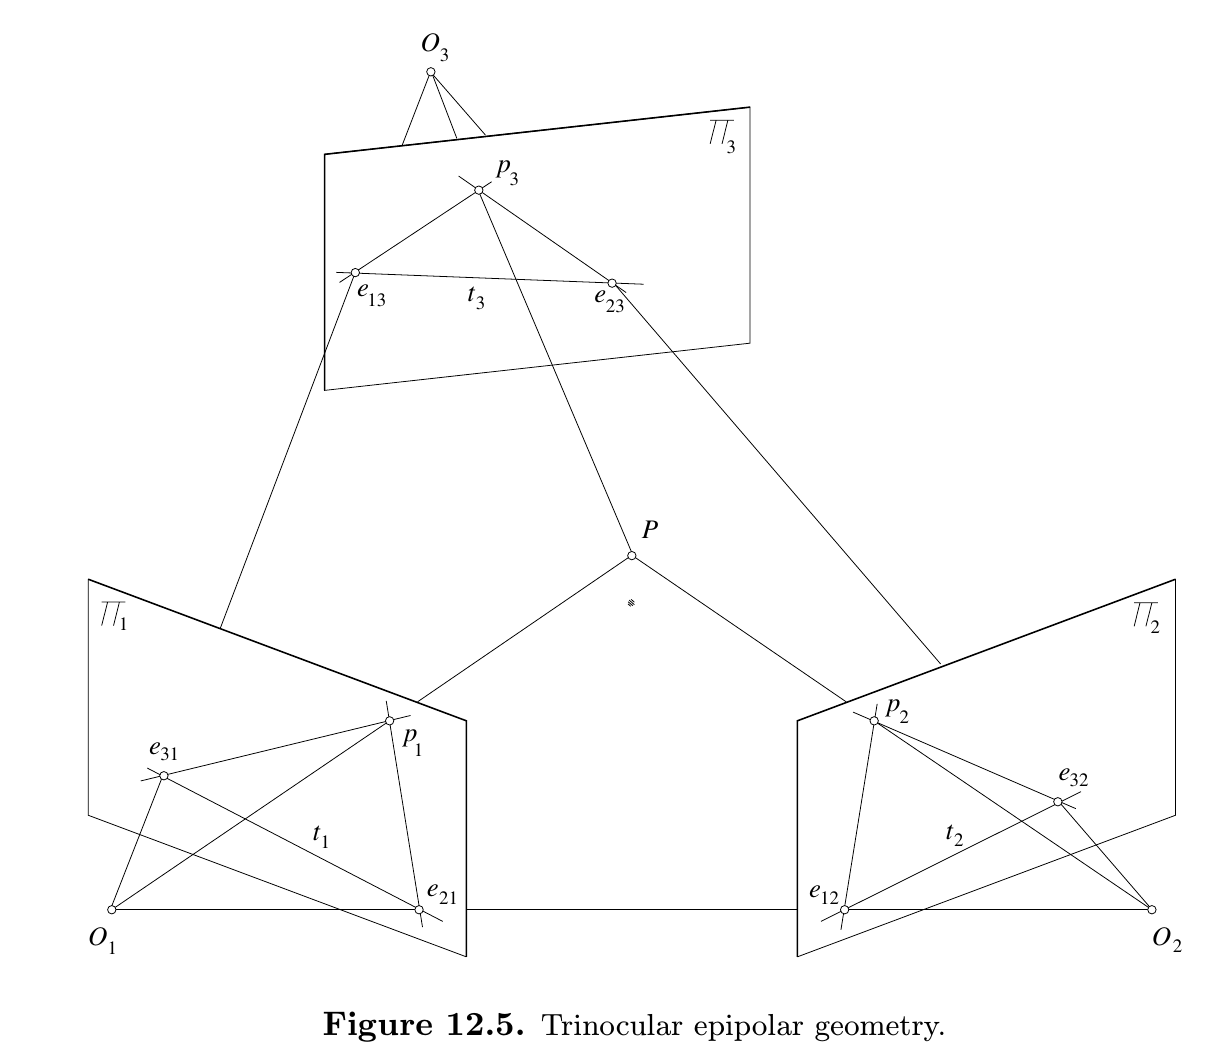
\includegraphics{img/trinocular_epipolar.png}}
\end{frame}}{\begin{frame}
  \frametitle{三目对极几何}
  \begin{eqnarray*}
    \tmmathbf{p}^T_1 \mathcal{E}_{12} \tmmathbf{p}_2 & = & 0\\
    \tmmathbf{p}^T_2 \mathcal{E}_{23} \tmmathbf{p}_3 & = & 0\\
    \tmmathbf{p}^T_3 \mathcal{E}_{31} \tmmathbf{p}_1 & = & 0
  \end{eqnarray*}
\end{frame}}{\begin{frame}
  \frametitle{直线}
  
  {\hspace{4em}}\resizebox{0.7\columnwidth}{!}{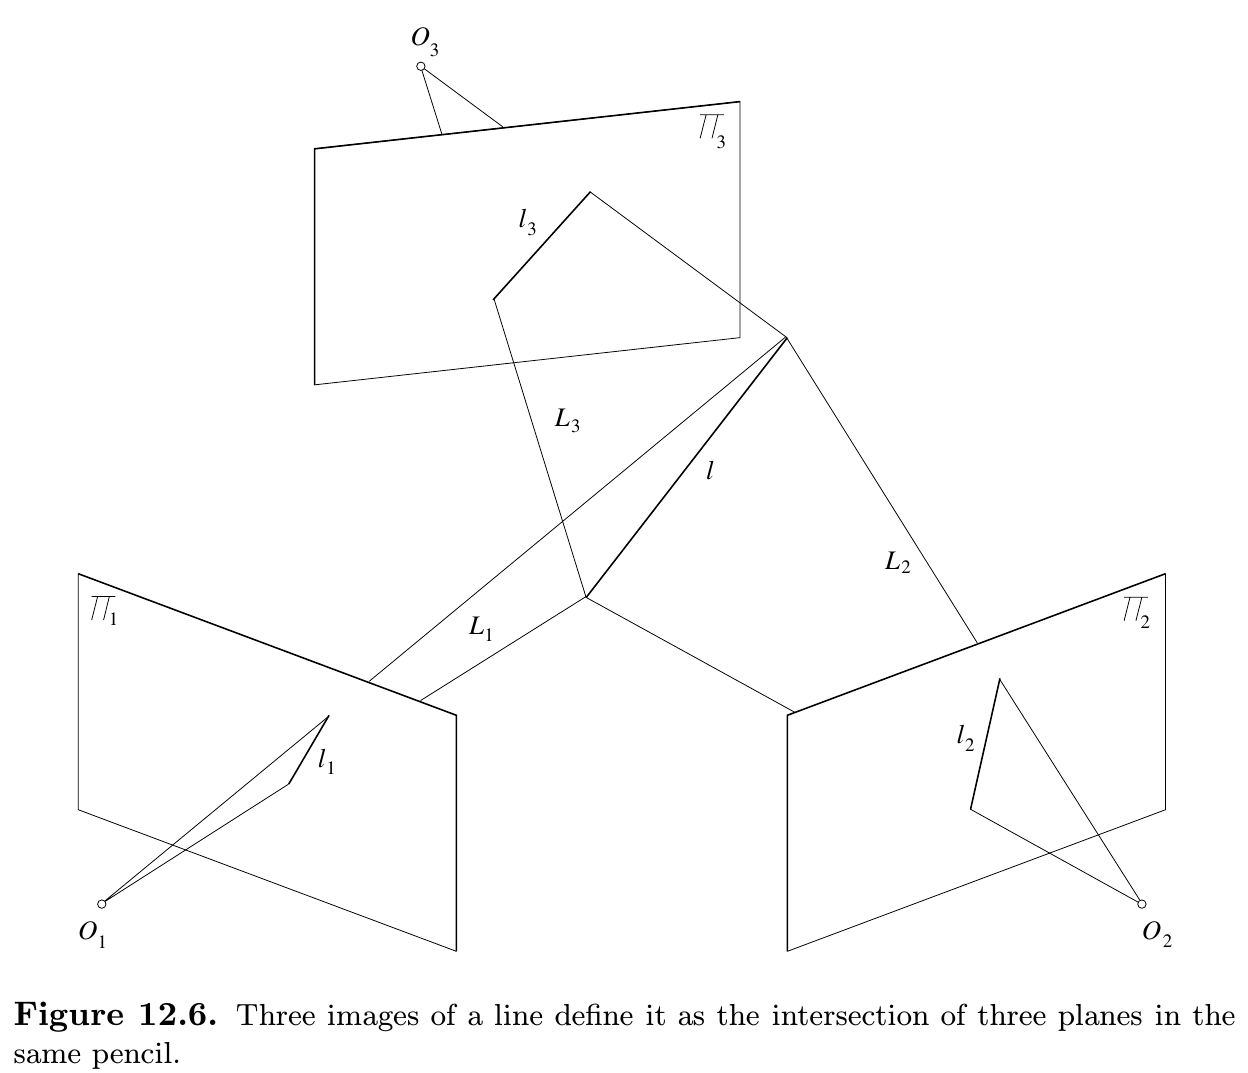
\includegraphics{img/three_image_lines_intersection.png}}
\end{frame}}{\begin{frame}
  \frametitle{三焦几何}
  \begin{eqnarray*}
    \tmmathbf{l}^T \mathcal{M}\tmmathbf{P} & = & \tmmathbf{0}
  \end{eqnarray*}
  得
  \begin{eqnarray*}
    \mathcal{L}\tmmathbf{P} & = & \tmmathbf{0}\\
    \mathcal{L} & \equiv & \left(\begin{array}{c}
      \tmmathbf{l}_1^T \mathcal{M}_1\\
      \tmmathbf{l}_2^T \mathcal{M}_2\\
      \tmmathbf{l}_3^T \mathcal{M}_3
    \end{array}\right)\\
    & = & \left(\begin{array}{c}
      \tmmathbf{L}_1^T\\
      \tmmathbf{L}_2^T\\
      \tmmathbf{L}_3^T
    \end{array}\right)\\
    \tmmathbf{L}_i & = & \mathcal{M}^T \tmmathbf{l}_i
  \end{eqnarray*}
\end{frame}}{\begin{frame}
  \frametitle{已标定情况}
  \begin{eqnarray*}
    \mathcal{M}_1 & = & \left(\begin{array}{cc}
      \tmmathbf{I} & \tmmathbf{0}
    \end{array}\right)\\
    \mathcal{M}_2 & = & \left(\begin{array}{cc}
      \mathcal{R}_2 & \tmmathbf{t}_2
    \end{array}\right)\\
    \mathcal{M}_1 & = & \left(\begin{array}{cc}
      \mathcal{R}_3 & \tmmathbf{t}_3
    \end{array}\right)
  \end{eqnarray*}
  得
  \begin{eqnarray*}
    \mathcal{L} & = & \left(\begin{array}{cc}
      \tmmathbf{l}_1^T & 0\\
      \tmmathbf{l}_2^T \mathcal{R}_2 & \tmmathbf{l}_2^T \tmmathbf{t}_2\\
      \tmmathbf{l}_3^T \mathcal{R}_3 & \tmmathbf{l}_3^T \tmmathbf{t}_3
    \end{array}\right)\\
    & = & \left(\begin{array}{cccc}
      \tmmathbf{l}_1^1 & \tmmathbf{l}_1^2 & \tmmathbf{l}_1^3 & 0\\
      \tmmathbf{l}_2^T \mathcal{R}_2^1 & \tmmathbf{l}_2^T \mathcal{R}_2^2 &
      \tmmathbf{l}_2^T \mathcal{R}_2^3 & \tmmathbf{l}_2^T \tmmathbf{t}_2\\
      \tmmathbf{l}_3^T \mathcal{R}_3^1 & \tmmathbf{l}_3^T \mathcal{R}_3^2 &
      \tmmathbf{l}_3^T \mathcal{R}_3^3 & \tmmathbf{l}_3^T \tmmathbf{t}_3
    \end{array}\right)
  \end{eqnarray*}
\end{frame}}{\begin{frame}
  \begin{eqnarray*}
    \left|\begin{array}{ccc}
      \tmmathbf{l}_1^2 & \tmmathbf{l}_1^3 & 0\\
      \tmmathbf{l}_2^T \mathcal{R}_2^2 & \tmmathbf{l}_2^T \mathcal{R}_2^3 &
      \tmmathbf{l}_2^T \tmmathbf{t}_2\\
      \tmmathbf{l}_3^T \mathcal{R}_3^2 & \tmmathbf{l}_3^T \mathcal{R}_3^3 &
      \tmmathbf{l}_3^T \tmmathbf{t}_3
    \end{array}\right| & = & 0\\
    \tmmathbf{l}_1^2 (\tmmathbf{l}_2^T \mathcal{R}_2^3 \tmmathbf{l}_3^T
    \tmmathbf{t}_3 -\tmmathbf{l}_3^T \mathcal{R}_3^3 \tmmathbf{l}_2^T
    \tmmathbf{t}_2) -\tmmathbf{l}_1^3 (\tmmathbf{l}_2^T \mathcal{R}_2^2
    \tmmathbf{l}_3^T \tmmathbf{t}_3 -\tmmathbf{l}_3^T \mathcal{R}_3^2
    \tmmathbf{l}_2^T \tmmathbf{t}_2) & = & 0\\
    \tmmathbf{l}_1^2 (\tmmathbf{l}_2^T \mathcal{R}_2^3 \tmmathbf{t}_3^T
    \tmmathbf{l}_3 -\tmmathbf{l}_2^T \tmmathbf{t}_2 \mathcal{R}_3^{3 T}
    \tmmathbf{l}_3) -\tmmathbf{l}_1^3 (\tmmathbf{l}_2^T \mathcal{R}_2^2
    \tmmathbf{t}_3^T \tmmathbf{l}_3 -\tmmathbf{l}_2^T \tmmathbf{t}_2
    \mathcal{R}_3^{2 T} \tmmathbf{l}_3) & = & 0\\
    \tmmathbf{l}_1^2 [\tmmathbf{l}_2^T (\mathcal{R}_2^3 \tmmathbf{t}_3^T
    -\tmmathbf{t}_2 \mathcal{R}_3^{3 T}) \tmmathbf{l}_3] -\tmmathbf{l}_1^3
    [\tmmathbf{l}_2^T (\mathcal{R}_2^2 \tmmathbf{t}_3^T -\tmmathbf{t}_2
    \mathcal{R}_3^{2 T}) \tmmathbf{l}_3] & = & 0\\
    \left|\begin{array}{ccc}
      \tmmathbf{l}_1^1 & \tmmathbf{l}_1^3 & 0\\
      \tmmathbf{l}_2^T \mathcal{R}_2^1 & \tmmathbf{l}_2^T \mathcal{R}_2^3 &
      \tmmathbf{l}_2^T \tmmathbf{t}_2\\
      \tmmathbf{l}_3^T \mathcal{R}_3^1 & \tmmathbf{l}_3^T \mathcal{R}_3^3 &
      \tmmathbf{l}_3^T \tmmathbf{t}_3
    \end{array}\right| & = & 0\\
    \left|\begin{array}{ccc}
      \tmmathbf{l}_1^1 & \tmmathbf{l}_1^2 & 0\\
      \tmmathbf{l}_2^T \mathcal{R}_2^1 & \tmmathbf{l}_2^T \mathcal{R}_2^2 &
      \tmmathbf{l}_2^T \tmmathbf{t}_2\\
      \tmmathbf{l}_3^T \mathcal{R}_3^1 & \tmmathbf{l}_3^T \mathcal{R}_3^2 &
      \tmmathbf{l}_3^T \tmmathbf{t}_3
    \end{array}\right| & = & 0
  \end{eqnarray*}
  
\end{frame}}{\begin{frame}
  \frametitle{三焦张量}
  
  
  \begin{eqnarray*}
    \tmmathbf{l}_1 \times \left(\begin{array}{c}
      \tmmathbf{l}_2^T \mathcal{G}_1^1 \tmmathbf{l}_3\\
      \tmmathbf{l}_2^T \mathcal{G}_1^2 \tmmathbf{l}_3\\
      \tmmathbf{l}_2^T \mathcal{G}_1^3 \tmmathbf{l}_3
    \end{array}\right) & = & \tmmathbf{0}\\
    \mathcal{G}_1^i & = & \tmmathbf{t}_2 \tmmathbf{R}_3^{i \nospace T}
    -\tmmathbf{R}_2^i \tmmathbf{t}_3^T \qquad i = 1, 2, 3
  \end{eqnarray*}
  
\end{frame}}{\begin{frame}
  
  \begin{eqnarray*}
    \tmmathbf{l}_1 & \propto & \left(\begin{array}{c}
      \tmmathbf{l}_2^T \mathcal{G}_1^1 \tmmathbf{l}_3\\
      \tmmathbf{l}_2^T \mathcal{G}_1^2 \tmmathbf{l}_3\\
      \tmmathbf{l}_2^T \mathcal{G}_1^3 \tmmathbf{l}_3
    \end{array}\right)\\
    \tmmathbf{p}_1^T \left(\begin{array}{c}
      \tmmathbf{l}_2^T \mathcal{G}_1^1 \tmmathbf{l}_3\\
      \tmmathbf{l}_2^T \mathcal{G}_1^2 \tmmathbf{l}_3\\
      \tmmathbf{l}_2^T \mathcal{G}_1^3 \tmmathbf{l}_3
    \end{array}\right) & = & 0
  \end{eqnarray*}
  where
  \begin{eqnarray*}
    \tmmathbf{P} & \in & \tmmathbf{l}\\
    \tmmathbf{p}_1 & = & \mathcal{M}_1 \tmmathbf{P}\\
    \tmmathbf{p}_1 & \in & \tmmathbf{l}_1\\
    \tmmathbf{p}_1 \tmmathbf{l}_1 & = & 0
  \end{eqnarray*}
\end{frame}}{\begin{frame}
  {\hspace{4em}}\resizebox{0.7\columnwidth}{!}{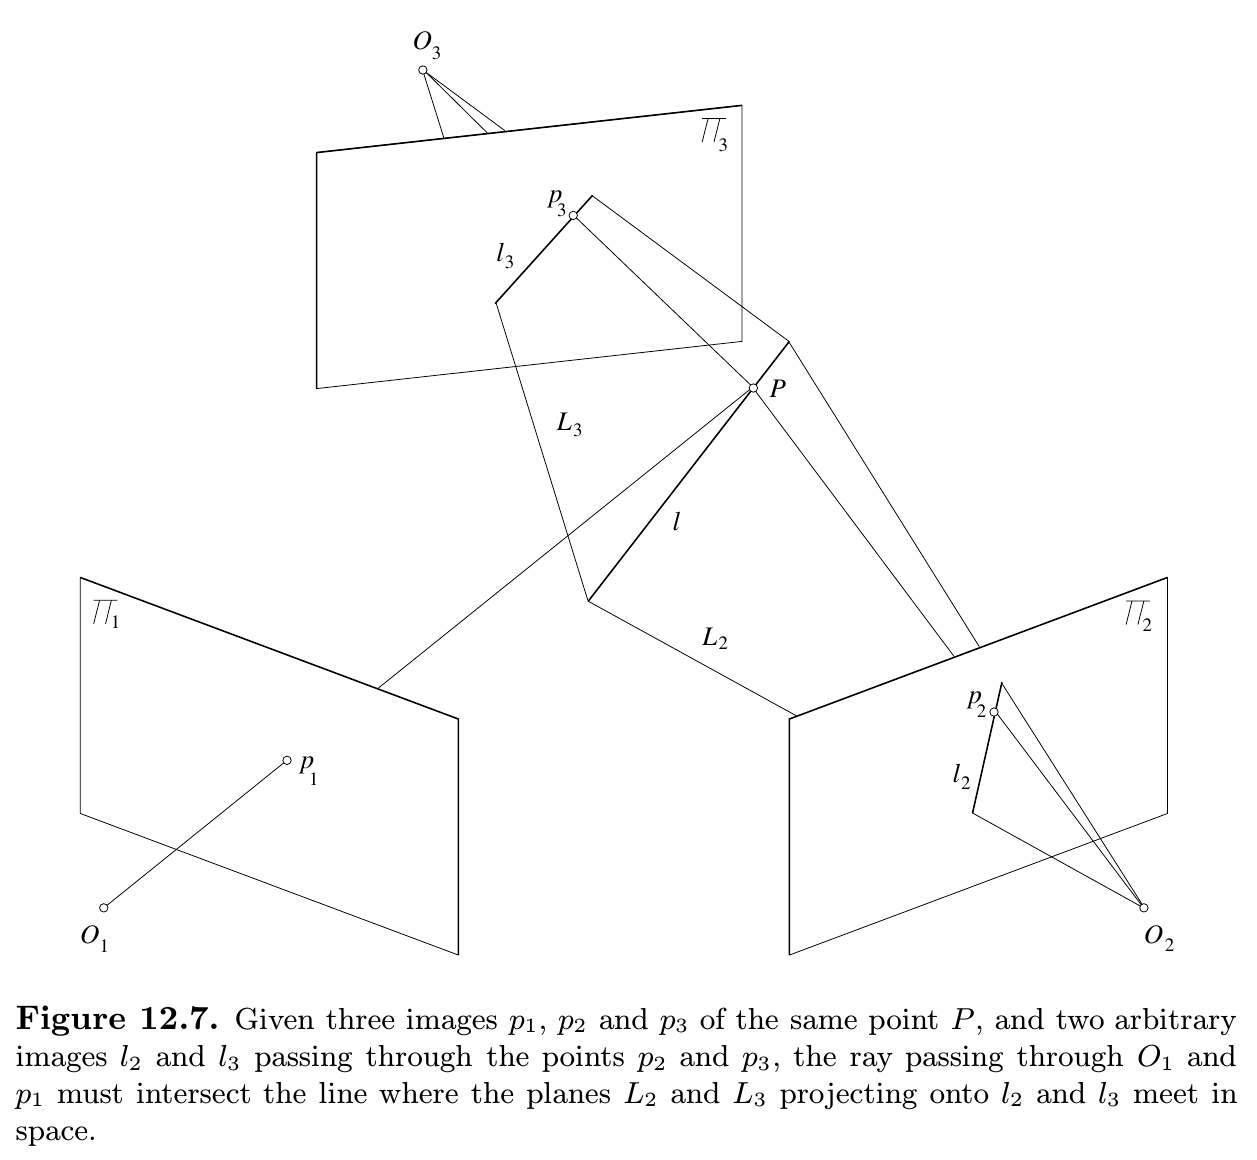
\includegraphics{img/three_image_point_lines.png}}
\end{frame}}{\begin{frame}
  \frametitle{未标定情况}
  \begin{eqnarray*}
    \tmmathbf{p} & = & \mathcal{K} \hat{\tmmathbf{p}}\\
    \tmmathbf{l}^T \tmmathbf{p} & = & 0\\
    \tmmathbf{l}^T \mathcal{K} \hat{\tmmathbf{p}} & = & 0
  \end{eqnarray*}
  得
  \begin{eqnarray*}
    \mathcal{L} & = & \left(\begin{array}{cc}
      \tmmathbf{l}_1^T \mathcal{K}_1 & 0\\
      \tmmathbf{l}_2^T \mathcal{K}_2 \mathcal{R}_2 & \tmmathbf{l}_2^T
      \mathcal{K}_2 \tmmathbf{t}_2\\
      \tmmathbf{l}_3^T \mathcal{K}_3 \mathcal{R}_3 & \tmmathbf{l}_3^T
      \mathcal{K}_3 \tmmathbf{t}_3
    \end{array}\right)
  \end{eqnarray*}
\end{frame}}{\begin{eqnarray*}
  \mathcal{L} \left(\begin{array}{cc}
    \mathcal{K}_1^{- 1} & \tmmathbf{0}\\
    \tmmathbf{0} & 1
  \end{array}\right) & = & \left(\begin{array}{cc}
    \tmmathbf{l}_1^T & 0\\
    \tmmathbf{l}_2^T \mathcal{A}_2 & \tmmathbf{l}_2^T \tmmathbf{b}_2\\
    \tmmathbf{l}_3^T \mathcal{A}_3 & \tmmathbf{l}_3^T \tmmathbf{b}_3
  \end{array}\right)\\
  \mathcal{A}_i & \equiv & \mathcal{K}_i \mathcal{R}_i \mathcal{K}_1^{- 1}\\
  \tmmathbf{b}_i & = & \mathcal{K}_i \tmmathbf{t}_i \qquad i = 2, 3
\end{eqnarray*}
对应
\begin{eqnarray*}
  \mathcal{M}_1 & = & \left(\begin{array}{cc}
    \mathcal{K}_1 & \tmmathbf{0}
  \end{array}\right)\\
  \mathcal{M}_2 & = & \left(\begin{array}{cc}
    \mathcal{A}_2 \mathcal{K}_1 & \tmmathbf{b}_2
  \end{array}\right)\\
  \mathcal{M}_3 & = & \left(\begin{array}{cc}
    \mathcal{A}_3 \mathcal{K}_1 & \tmmathbf{b}_3
  \end{array}\right)
\end{eqnarray*}
且有
\begin{eqnarray*}
  \mathcal{G}_1^i & = & \tmmathbf{b}_2 \tmmathbf{A}_3^{i \nospace T}
  -\tmmathbf{A}_2^i \tmmathbf{b}_3^T\\
  \mathcal{A}_i & = & \left(\begin{array}{ccc}
    \tmmathbf{A}^1_i & \tmmathbf{A}_i^2 & \tmmathbf{A}_i^3
  \end{array}\right)
\end{eqnarray*}}}

\end{document}
